\documentclass[tikz, border=10pt]{standalone}
\usepackage{tikz}
\usetikzlibrary{shapes.multipart, positioning, arrows.meta, calc}

\begin{document}
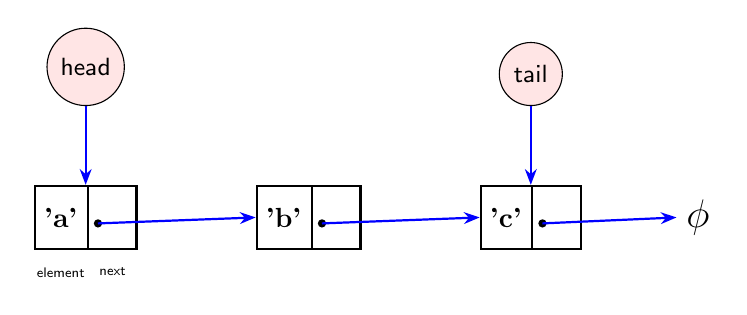
\begin{tikzpicture}[
    listnode/.style={
        rectangle split,
        rectangle split parts=2,
        rectangle split horizontal,
        draw,
        thick,
        fill=white,
        minimum height=0.8cm,
        rectangle split part fill={white, gray!10}
    },
    ptr/.style={
        >={Stealth[length=2mm]},
        ->,
        thick,
        blue
    },
    headtail/.style={
        draw, 
        circle, 
        fill=red!10, 
        minimum size=0.8cm,
        font=\small\sffamily
    },
    label/.style={
        font=\small\sffamily
    }
]

    % Nodes
    % \nodepart{one} is default
    \node[listnode] (node1) { \textbf{'a'} \nodepart{two} \phantom{xx}};
    \node[listnode, right=1.5cm of node1] (node2) { \textbf{'b'} \nodepart{two} \phantom{xx}};
    \node[listnode, right=1.5cm of node2] (node3) { \textbf{'c'} \nodepart{two} \phantom{xx}};
    \node[right=1.2cm of node3, font=\Large] (null) {$\phi$};

    % Dots in the pointer fields help visualize origin
    \fill[black] (node1.two) circle (1.5pt);
    \fill[black] (node2.two) circle (1.5pt);
    \fill[black] (node3.two) circle (1.5pt);

    % Pointers connecting nodes
    \draw[ptr] (node1.two) -- (node2.west);
    \draw[ptr] (node2.two) -- (node3.west);
    \draw[ptr] (node3.two) -- (null.west);

    % Head Pointer
    \node[headtail, above=1cm of node1] (head) {head};
    \draw[ptr] (head) -- (node1.north);

    % Tail Pointer
    \node[headtail, above=1cm of node3] (tail) {tail};
    \draw[ptr] (tail) -- (node3.north);

    % Field Labels on first node
    \node[below=0.1cm of node1.one south, font=\tiny\sffamily] {element};
    \node[below=0.1cm of node1.two south, font=\tiny\sffamily] {next};
    
\end{tikzpicture}
\end{document}
